\documentclass[12pt, a4paper]{article}
\usepackage{scrextend}
\usepackage[utf8]{inputenc}
\usepackage[polish]{babel}
\usepackage[T1]{fontenc}%polskie znaki
\usepackage[utf8]{inputenc}%polskie znaki
\usepackage{geometry}
\usepackage{float}
\usepackage{enumitem}
\usepackage{hyperref}
\usepackage{graphicx}
\usepackage{amsmath}
\usepackage{tabularx}
\usepackage{pdflscape}


\renewcommand{\baselinestretch}{1.5}


\begin{document}

\begin{flushleft}
    Damian Koper \textbf{241292} \\
\end{flushleft}
\vspace{1cm}
{
    \centering
    {\Huge\scshape\bfseries Modelowanie i analiza systemów informatycznych }\\
    \large{Logika Temporalna i Automaty Czasowe - konstrukcja i weryfikacja czasowych automatów UPPAAL 1.}\\
    \vspace{0.5cm}
}
\newcounter{ex}
\setcounter{ex}{0}
\newcommand{\ex}[1]{
    \refstepcounter{ex}{
        \noindent\normalfont\Large\bfseries Zadanie \arabic{ex}.
    } \\
    #1
}

\ex{Czas i alarm}
\begin{figure}[H]
    \centering
    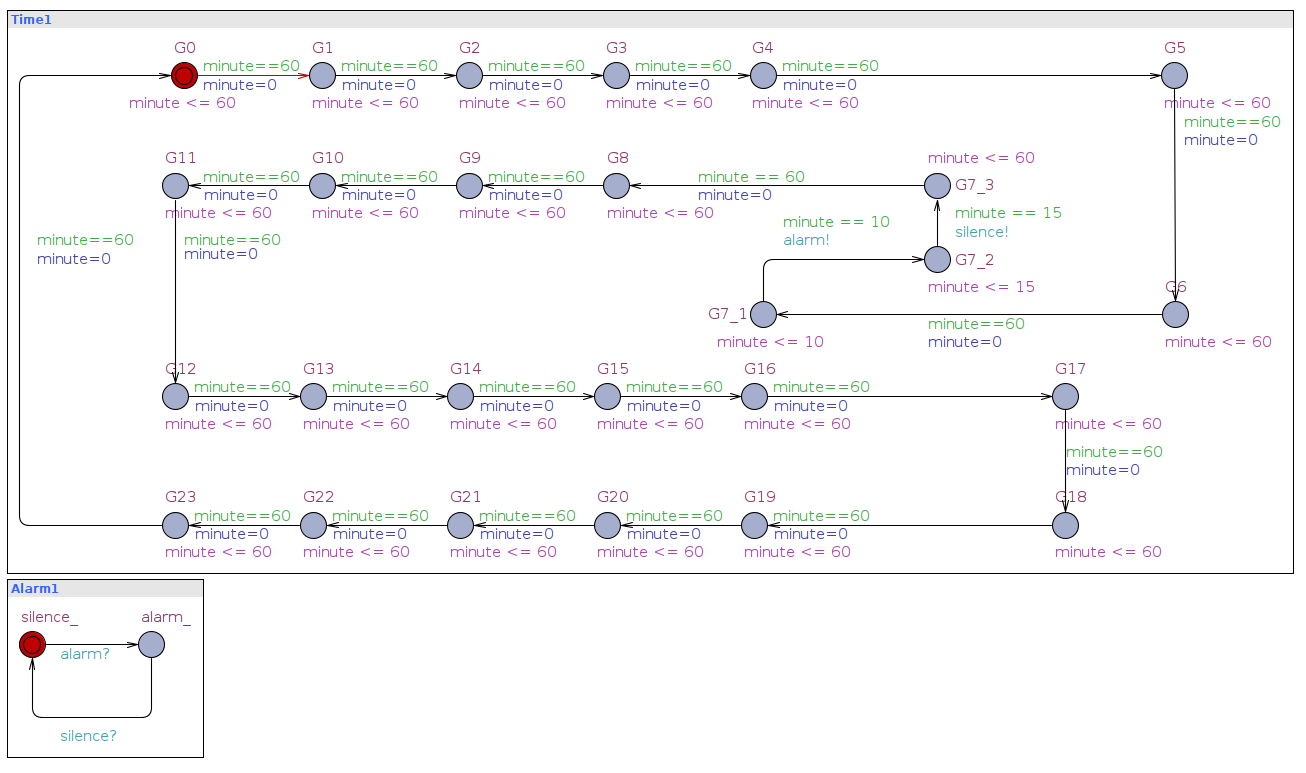
\includegraphics[width=\linewidth]{../../lab12/ex_1_2}
\end{figure}

\ex{Weryfikacja automatów z zadania 1}
\newgeometry{left=0cm,bottom=2cm,top=2cm,right=0cm}

\begin{landscape}
    \begin{table}
        \centering
        \begin{tabularx}{\linewidth}{X|X|X|l}
            \texttt{A[] T.G0 imply T.minute <= 60}                                          & AG(T.G0 $\implies$ T.minute $\le$ 60)                                                           & Na pewno zawsze w T.G0, minuta $\le$ 60                                   & True \\ \hline
            \texttt{A<> T.G0 and T.minute == 60}                                            & AF(T.G0 $ \wedge $ T.minute = 60)                                                               & Na pewno kiedyś w T.G0, minuta = 60                                       & True \\ \hline
            \texttt{A[] T.minute <= 60}                                                     & AG(T.minute <= 60)                                                                              & Na pewno zawsze minuta $\le$ 60                                           & True \\ \hline
            \texttt{A<> T.minute == 60}                                                     & AF(T.minute = 60)                                                                               & Na pewno kiedyś minuta = 60                                               & True \\ \hline
            \texttt{T.G0 --> T.G23}                                                         & AG(T.G0 $\implies$ AF T.G23)                                                                    & Na pewno po T.G0 nastąpi kiedyś T.G23                                     & True \\ \hline
            \texttt{T.G23 --> T.G0}                                                         & AG(T.G23 $\implies$ AF T.G0)                                                                    & Na pewno po T.G0 nastąpi kiedyś T.G23                                     & True \\ \hline
            \texttt{A[] T.G7\_1 imply T.minute <= 10}                                       & AG(T.G7\_1 $\implies$ T.minute $\le$ 10)                                                        & Na pewno zawsze w T.G7\_1, minuta $\le$ 10                                & True \\ \hline
            \texttt{A<> T.G7\_1 and T.minute == 10}                                         & AF(T.G7\_1 $ \wedge $ T.minute = 10)                                                            & Na pewno kiedyś w T.G7\_1, minuta = 10                                    & True \\ \hline
            \texttt{A[] T.G7\_2 imply T.minute >= 10 and T.minute <= 15}                    & AG(T.G7\_2 $\implies$ T.minute $\ge$ 10 $ \wedge $ T.minute $\le$ 15)                           & Na pewno zawsze w T.G7\_2, minuta $\ge$ 10 i minuta $\le$ 15              & True \\ \hline
            \texttt{A<> T.G7\_2 and T.minute == 15}                                         & AF(T.G7\_2 $ \wedge $ T.minute = 15)                                                            & Na pewno kiedyś w T.G7\_2, minuta = 15                                    & True \\ \hline
            \texttt{A[] T.G7\_3 imply T.minute >= 15 and T.minute <= 60}                    & AG(T.G7\_3 $\implies$ T.minute $\ge$ 15 $ \wedge $ T.minute $\le$ 60)                           & Na pewno zawsze w T.G7\_3, minuta $\ge$ 15 i minuta $\le$ 60              & True \\ \hline
            \texttt{A<> T.G7\_3 and T.minute == 60}                                         & AF(T.G7\_3 $ \wedge $ T.minute = 60)                                                            & Na pewno kiedyś w T.G7\_3, minuta = 60                                    & True \\ \hline
            \texttt{A[] T.G7\_2 imply Alarm1.alarm\_}                                       & AG(T.G7\_2 $\implies$ Alarm1.alarm\_)                                                           & Na pewno zawsze w T.G7\_2, Alarm1.alarm\_                                 & True \\ \hline
            \texttt{A[] Alarm1.alarm\_ imply T.G7\_2 and T.minute >= 10 and T.minute <= 15} & AG(Alarm1.alarm\_ $\implies$ T.G7\_2 $ \wedge $ T.minute $\ge$ 10 $ \wedge $  T.minute $\le$ 15 & Na pewno zawsze w Alarm1.alarm\_, będzie w T.G7\_2 i minute $\in$ [10,15] & True \\ \hline
            \texttt{A<> Alarm1.alarm\_ and T.G7\_2 and T.minute == 15}                      & AF(Alarm1.alarm\_ $ \wedge $ T.G7\_2 $ \wedge $  T.minute = 15                                  & Na pewno kiedyś  Alarm1.alarm\_ i T.G7\_2 i minuta == 15                  & True \\
        \end{tabularx}
        \caption{Formuły weryfikacyjne. Automat ma tylko jedną ścieżkę (cykl), więc użyto tylko operatora A}
    \end{table}
\end{landscape}
\restoregeometry
\end{document}
